\documentclass[12pt, letterpaper]{article}
\usepackage[utf8]{inputenc}
\usepackage[margin=2cm]{geometry}
\usepackage{amsmath}
\usepackage{amssymb}
\usepackage{graphicx}
\usepackage{cancel}
\usepackage{fancyhdr}
\usepackage{float}

\graphicspath{ {./bilder/} }

\title{ \begin{huge}
\textbf{Portfolio Assignment 3}
\end{huge} }

\author{Candidate 25}
\date{}

\rfoot{\thepage}
\newcommand{\bs}{\boldsymbol}
\newcommand{\mbf}{\mathbf}

\begin{document}
\maketitle
  \section*{Problem 1}
    \subsection*{(1a)}
      I shall now discuss the main difference between feature extraction and feature selection.\\

      In both feature seletion and extraction the goal is to reduce the dimensionality of the dataset. Theese are both categories which do this differently. Both algorithms are used to try and avoid the \textit{curse of dimensionality}, a term used to describe the problem of searching for patterns in data which span many features.\\
      In feature extraction we reduce the dimensionality by creating new sets of data, based on the original dataset, this can be done with methods such as principal component analysis or what I am going to do in this problem, multidimensional scaling.\\
      In feature selection we wish to choose features of a dataset which does a good job of describing the dataset as a whole. Sometimes an approach to this would be to look at the correlation between features, such that if two features have are highly correlated, then choose the feature which best represent the two.\\

      In this problem I implemented a program which used the multidimensional scaling (MDS) algorithm, to reduce the number of dimensions in the final output. The way MDS works is by using a result from linear algebra known as eigendecomposition, which uses the eigenvalues and eigenvectors to make what might have began as data structured with 10 features and many datapoints, into data with only 2 or 3 features.\\
      If we define our dataset $X$ we can use eigendecomposition which gives the matrix $E$ which consist of the eigenvectors put together as columnvectors, and the matrix $D$ which is a diagonalmatrix with only eigenvalues on it's main diagonal.
      \begin{align*}
        X^T X = EDE^T &= ED^{1/2}D^{1/2}E^T\\
        \text{IF: } Z &= D^{1/2}E^T\\
        \implies Z^T Z &= X^T X
      \end{align*}
      This means we have maximally preserved the inner products and $Z$ is a good representation of $X$. Now we can choose how many dimensions we wish to use. We do this by choosing $k \geq 1$ dimensions and then determining the $k$ largest eigenvalues $\lambda_1, ..., \lambda_k$ of the $n \times n$ eigenvalue matrix $D$, and the corresponding eigenvectors $e_1, ..., e_k$ of the $n \times n$ matrix $E$ of eigenvectors.
    \subsection*{(1b)}
      In this task we are interested in reducing a 34 x 34 matrix which contains the geodesic distances between 34 swedish cities, into something we can plot on a two dimensional map.\\
      To do this we use MDS and specify that we only want 2 dimensions on the resulting coordinate matrix. The algorithm is naturally capable of not only reducing to two dimensions but any dimension smaller than the original dimension of the dataset. We could for instance using some sort of spherical coordinate system, first reduce the dataset to three dimensions, then project them on the surface of some earth-like ellipsoid. But for our purpose we only need two dimensions to illustrate a map of the Swedish cities.\\
    \subsection*{(1c)}
      \begin{figure}[H]
        \caption{Resulting 2 dimensional plot of 34 Swedish cities.}
        \centering
        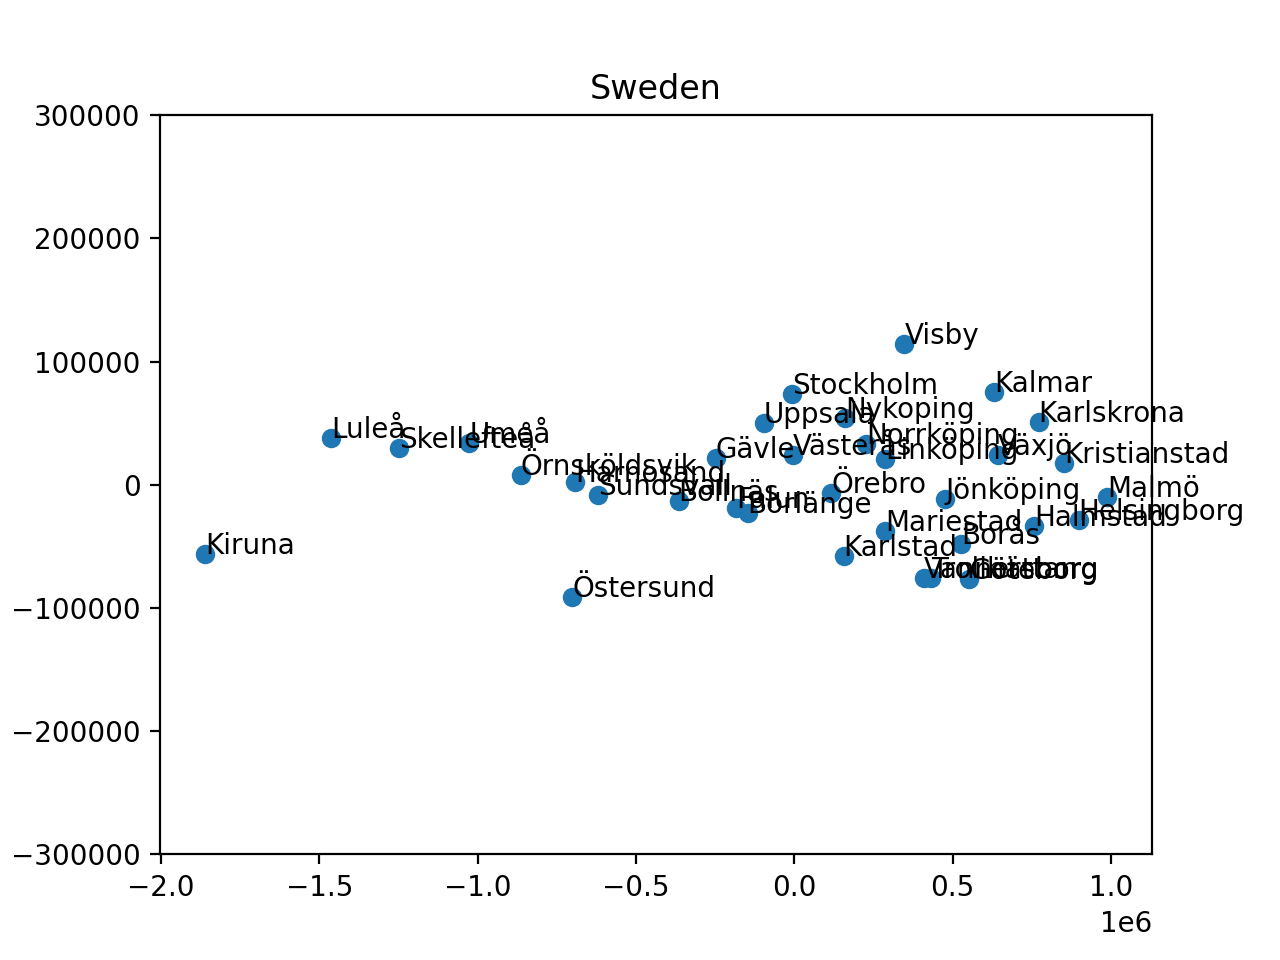
\includegraphics[scale=0.7]{Swedishcities}
        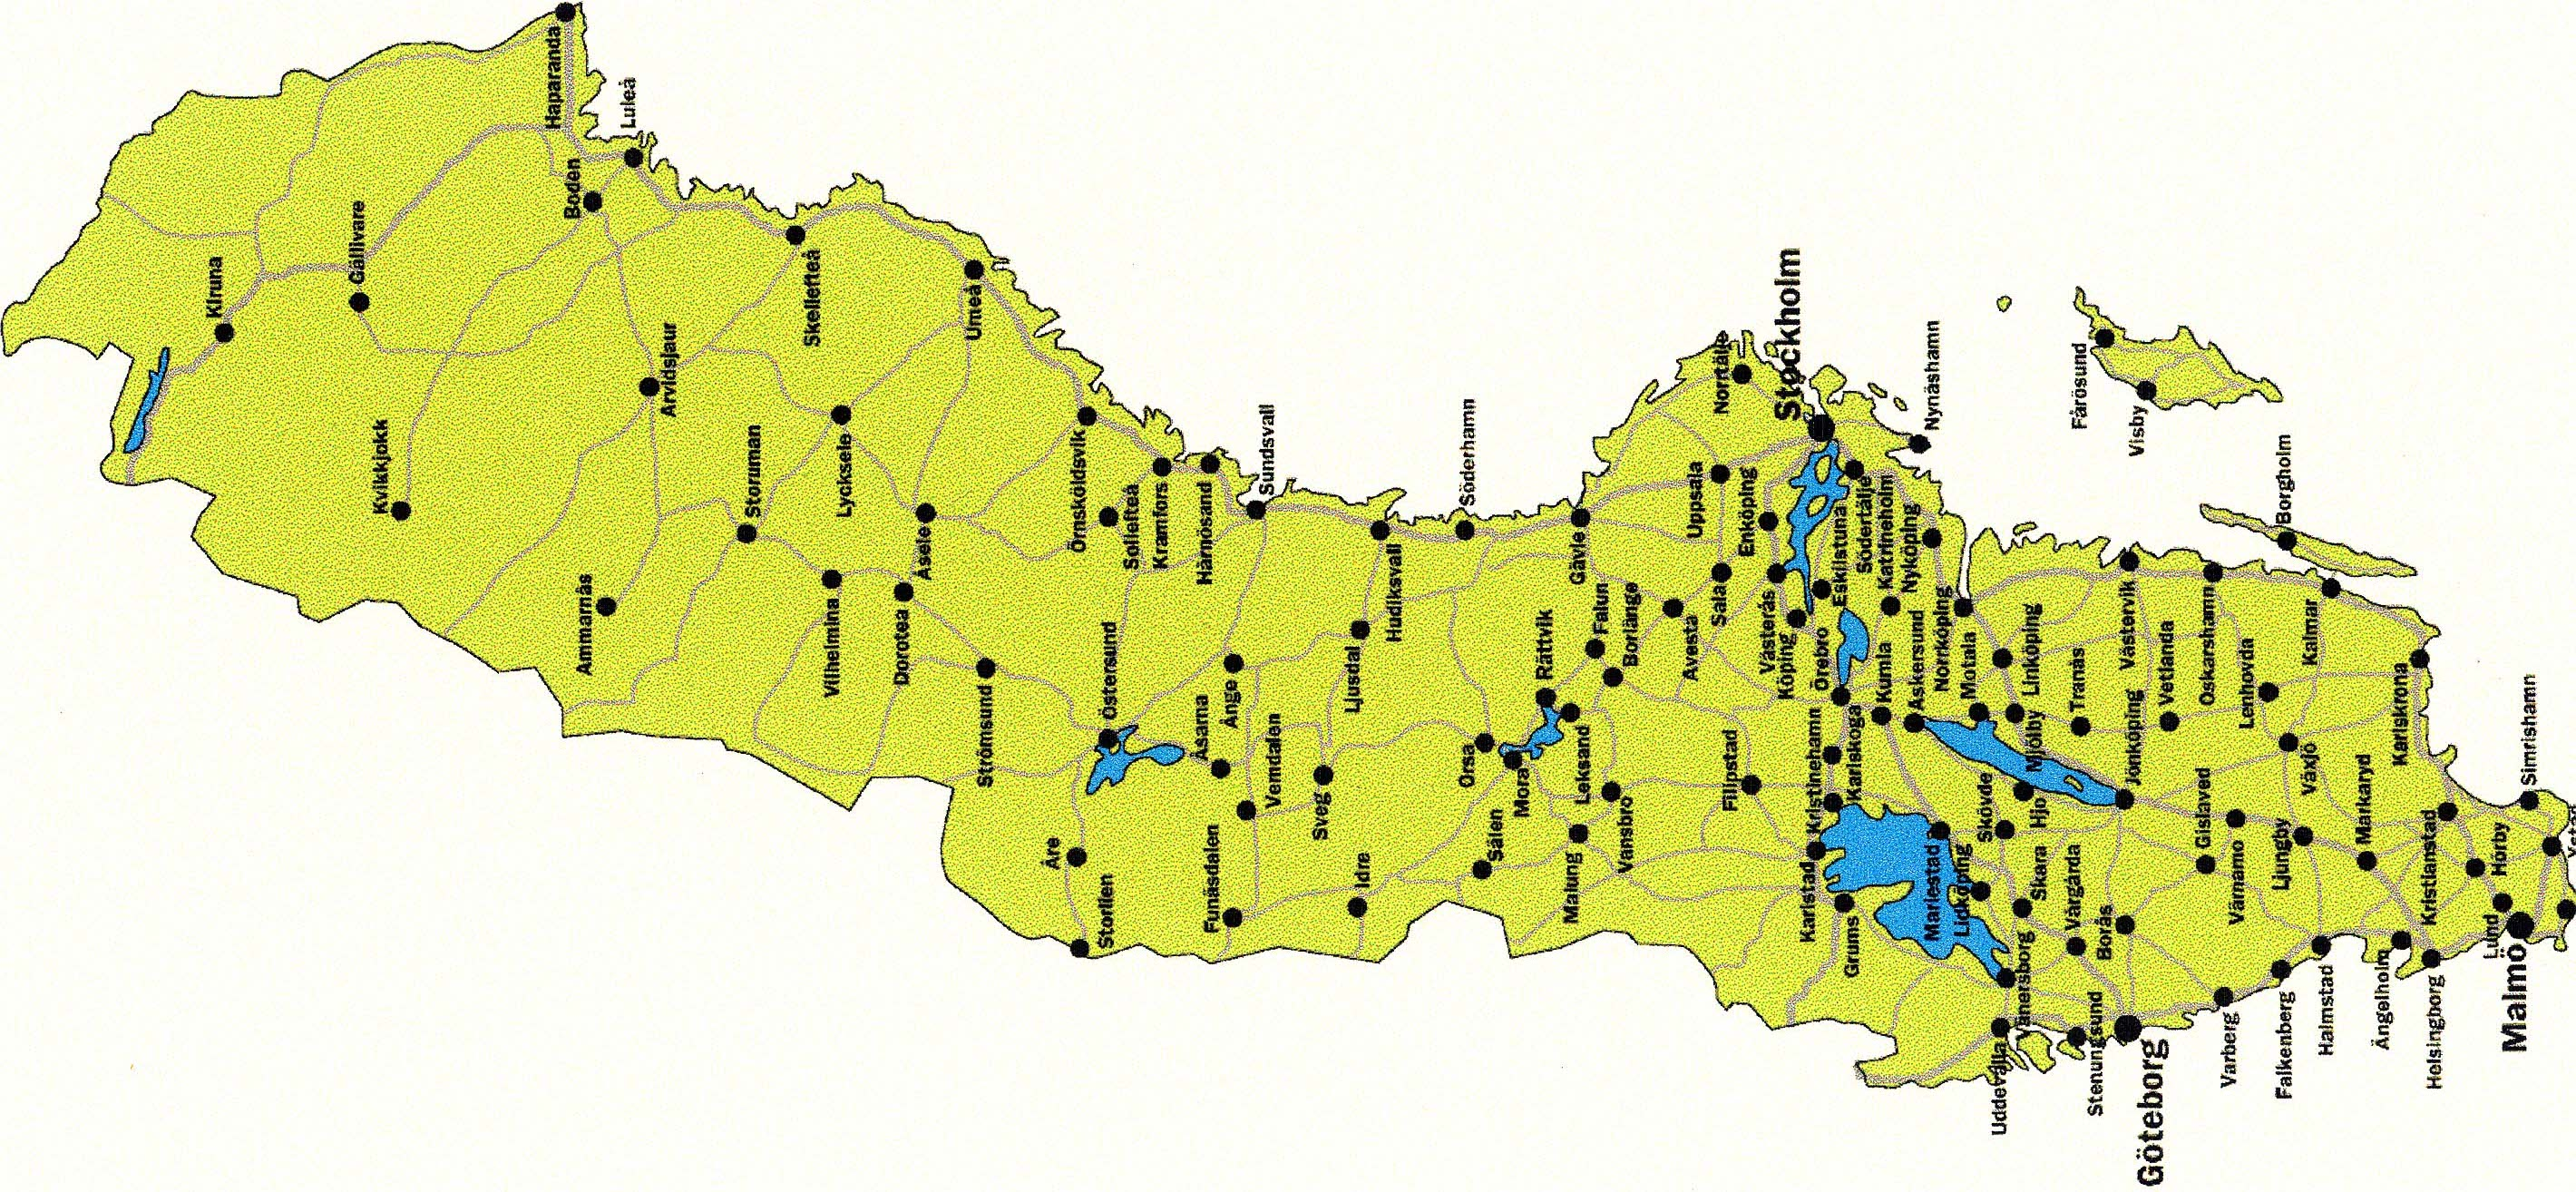
\includegraphics[scale=0.1]{Swedishmap}
      \end{figure}
      Here we clearly see the similarities althoug the city names of the actual swedish map is too tiny to distinguish from the background. The axes of the plot do not describe the real distances between the cities but have a relation such that theese distances are proportional to the real distances. This means the distances in the data are relationally correct to each other.
      Originally the plot did not look this nice, but I have manually scaled the second axis such that it resembles the map of sweden better.\\
  \section*{Problem 2}
    \subsection*{(2a)}
      The k-means algorithm is an unsupervised iterative machine learning method for finding clusters in a dataset which does not have a ground truth to compare against. The first step in this algorithm is to find k random vectors which preferably lay in the domain of the dataset. This is where we first initialize the algorithm. There are some problems which can present themselves based on our initial choice of k random vectors. I will come to theese problems when I have presented the algorithm as a whole.\\
      Now there have been generated k random vectors, which we can call clusters. The algorithm then checks which datapoints lay closest to theese clusters. Now take the mean of all the datapoints that we found were closest to each cluster. Then move each cluster to the means we just found. The last step is to iteratively find the closest datapoints, find the means then move the cluster to theese means over and over again until the cluster dont move any more. Then the we say the algorithm has converged, and is done.\\
      The problems which I mentioned earlier with initializing the algorithm can appear if the first selection of random clusters are at a place not close to any actual groupings of datapoints, and there are some other cluster which is blocking it's path towards the data grouping. If this happens we are left with a false cluster which might be at the center of some sparsely populated area of the vector space in which the datapoints are.\\
      Another way the algorithm can fail is when groupings of data have a shape which dont resemlbe simple elliptical or similar shapes, but rater a cluster which span one axis in such a way that there is another cluster in between. I will illustrate this problem with this figure:\\
      \begin{figure}[H]
        \caption{Example plot where k-means algorithm does a good and a poor job.}
        \centering
        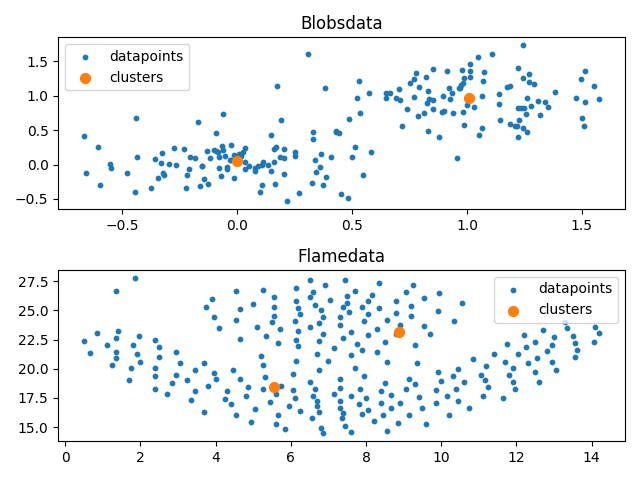
\includegraphics[scale=0.69]{exampleplot}
      \end{figure}
      The bottom of the two plots, with the title \textit{Flamedata} is from a previous assignment where I used the same algorithm. Here the bottom cluster does not represent the whole banana-like shaped grouping of data in a good way. While the top plot is an illustration where the k-means algorithm does a good job representing the clusters, since there are two distinct groupings of data which have this shape compatible with the algorithm.
    \subsection*{(2b)}
      In this problem I implement the k-means algorithm with $k = 2, k = 4$ and $k = 10$ clusters, theese are my plots. As you can see they are plotted in such a way where we have every other row as centroids and images closest to the centroids, and at the bottom I have plotted the border cases.
      \begin{figure}[H]
        \caption{$K = 2$ clusters.}
        \centering
        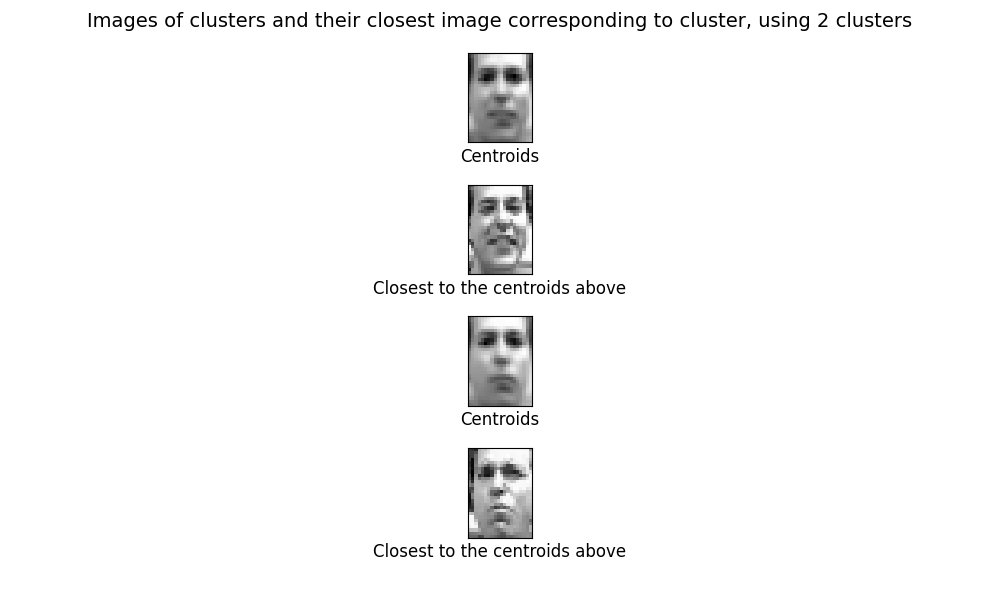
\includegraphics[scale=0.7]{cluster2}
        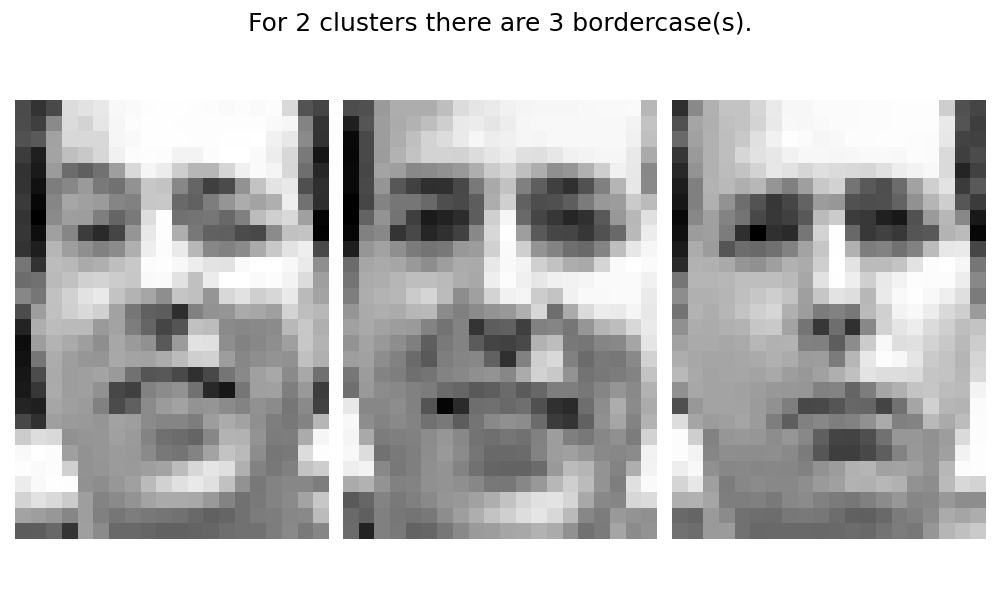
\includegraphics[scale=0.4]{border2}
      \end{figure}
      \begin{figure}[H]
        \caption{$K = 4$ clusters.}
        \centering
        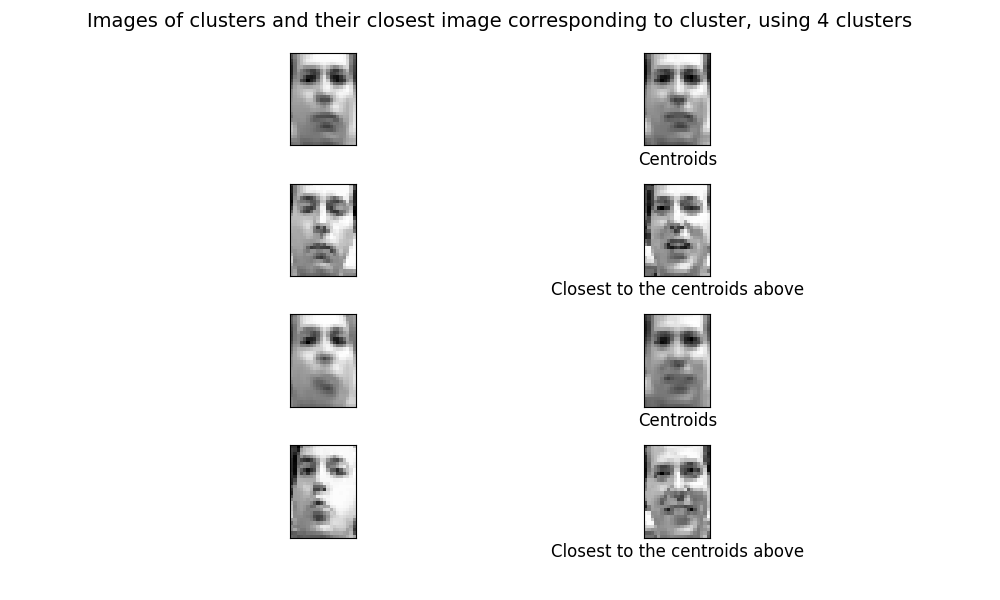
\includegraphics[scale=0.7]{cluster4}
        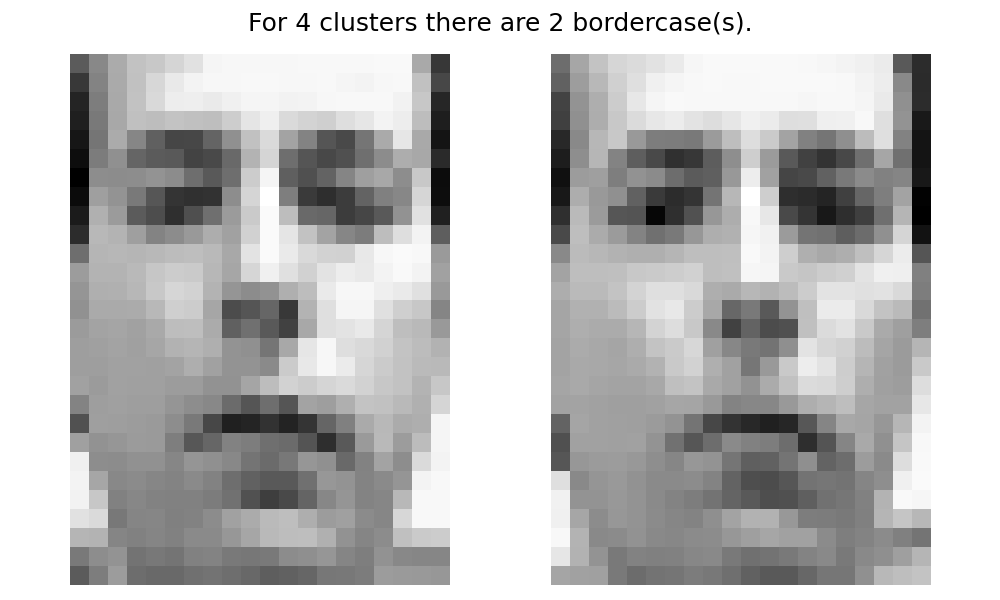
\includegraphics[scale=0.4]{border4}
      \end{figure}
      \begin{figure}[H]
        \caption{$K = 10$ clusters.}
        \centering
        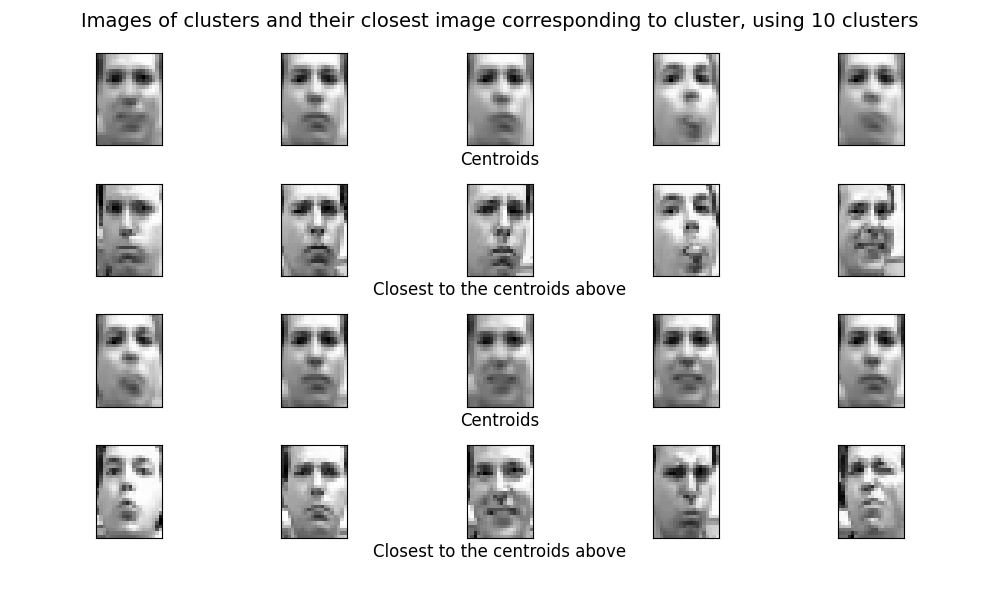
\includegraphics[scale=0.7]{cluster10}
        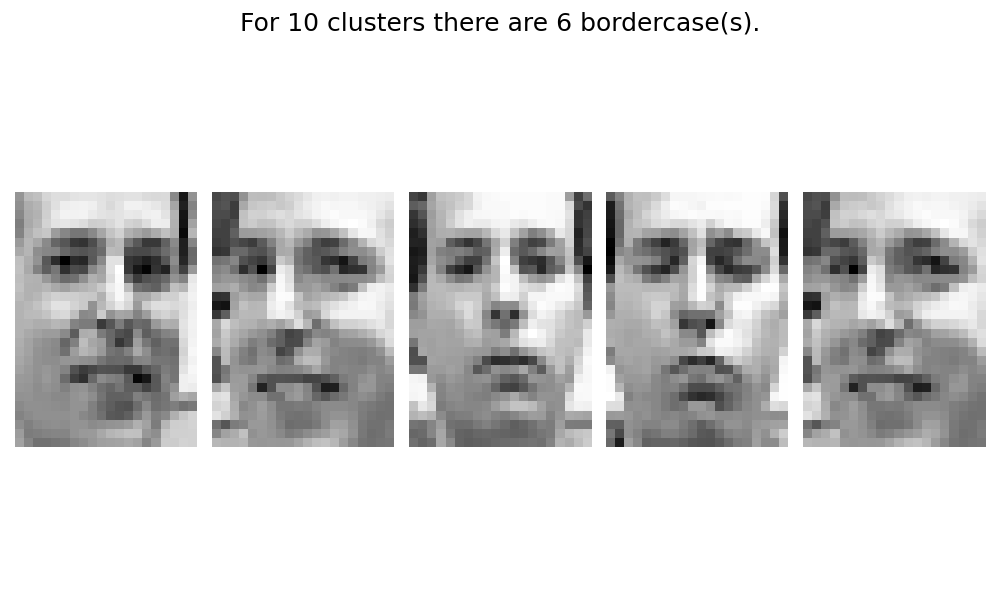
\includegraphics[scale=0.4]{border10}
      \end{figure}
    \subsection*{(2c)}
      For both structure and simplicity I plotted the bordercases underneath the cluster plots.\\
      For 2 clusters, it seems theese are the most general facial expressions from the dataset, with not too many outstanding features, which I think makes sense as theese are the most common expressions. It even seems as thoug the top centroid is the facial expression of happiness, and the bottom cluster is the expression of disgust or anger. The bordercase kind of look like a very neutral face, the kind of expression you have when strolling through a shopping mall.\\
      For 4 clusters we get a bit of a different but still similar result, here the two top clusters look like they are two versions of confusion, while the bottom left might represent some kind of disgust again and the bottom right represents joy. The bordercases also seem to be very neutral facial expressions.\\
      Using 10 clusters the result is more interesting. There are now not only the basic facial expressions but more complex expressions. Some are smiling, some are sad. Here the bordercases reveals again that the more neutral expressions seem to lay in between the clusters.
\end{document}
